\documentclass[12pt,a4paper]{article}
\usepackage{amsmath, amssymb}
\usepackage{geometry}
\usepackage{hyperref}
\usepackage{booktabs}
\usepackage{graphicx}
\usepackage{setspace}
\usepackage{listings}
\usepackage{titlesec}
\usepackage{tikz}
\usepackage{pgfplots}
\usepackage{xcolor}
\usepackage{float}
\lstset{
    language=Python,
    basicstyle=\ttfamily\small,
    numbers=left,
    numberstyle=\tiny,
    frame=tb,
    columns=fullflexible,
    showstringspaces=false,
    breaklines=true,
    keywordstyle=\color{blue},
    commentstyle=\color{green!60!black},
    stringstyle=\color{red}
}

\usepackage

\geometry{margin=1in}
\setcounter{secnumdepth}{3}
\graphicspath{{assets/}}

\begin{document}

% Title Page
\begin{titlepage}
    \centering
    
    \Huge
    \textbf{Jaypee Institute of Information Technology, Sector - 62, Noida } \\
    \vspace{0.5cm}
    \Large
    \textbf{Mathematics Project Report}\\
    \vspace{0.5cm}

    
    
\includegraphics[scale=0.2]{jiit_logo.png}\\
    
    \vspace{0.5cm}
    \Huge
    \textbf{Project Report}\\
    \Large
    
    \textbf{Analysis of Initial Value Problems: \\
    Mathematical Modeling, Numerical Methods, and Computational Approaches}\\
    \vspace{0.5cm}

    \Large
    \textbf{Submitted to}\\
    Dr.Manish Bansal \\
    Mathematics Department\\
    \vspace{1cm}

    \textbf{Submitted by}
    \vspace{0.5cm}

    \begin{tabular}{lll}
        Agnibha Nanda & B7 & 2401030306 \\
        Sansriti Mishra & B7 & 2401030293 \\
        Amogh Shukla & B7 & 2401030290 \\
        Sanvi Dhingra & B7 & 2401030309 \\
        Durlabh Thareja & B7 & 2401030305 \\
    \end{tabular}

    \vspace*{\fill}
    \normalsize
\end{titlepage}

% Letter of Transmittal
\begin{center}
    \Large\textbf{Letter of Transmittal}
\end{center}
\vspace{1cm}

\noindent
\textbf{Dr. Manish Bansal} \\
[0.5em]
Department of Mathematics \\
[0.5em]
Jaypee Institute of Information Technology \\
[0.5em]
\vspace{1cm}

\noindent
\textbf{Subject:} Submission of Project Report on ``Analysis of Initial Value Problems''

\vspace{1cm}

\noindent
Dear Sir,

\vspace{1em}

\noindent
We are pleased to submit our project report on Initial Value Problems (IVPs), which provides an in-depth exploration of mathematical modeling, numerical methods, and computational approaches for solving differential equations.

\vspace{1em}

\noindent
This report covers theoretical foundations, numerical techniques, computational implementations, and real-world applications of Initial Value Problems across various scientific disciplines.

\vspace{1em}

\noindent
We hope this project meets your academic expectations and demonstrates our understanding of the complex mathematical concepts involved.

\vspace{2em}

\noindent
Sincerely, \\[2em]

\noindent
    Agnibha Nanda (2401030306) \\
    Sansriti Mishra (2401030293) \\
    Amogh Shukla (2401030290) \\
    Sanvi Dhingra (2401030309) \\
    Durlabh Thareja (2401030305) \\

\vspace{2cm}

\noindent
Date: \today

\newpage

\tableofcontents

\newpage

\section{Abstract}
Initial Value Problems (IVPs) are fundamental mathematical models that describe the evolution of dynamic systems governed by differential equations. This comprehensive project provides an in-depth exploration of:

\begin{itemize}
    \item Advanced theoretical foundations of IVPs
    \item Comprehensive numerical solution techniques
    \item Sophisticated computational implementation strategies
    \item Detailed mathematical analysis and error estimation
    \item Diverse real-world applications across scientific domains
\end{itemize}

The research systematically investigates multiple solution approaches, emphasizing the intricate relationship between mathematical theory, numerical methods, and computational implementation.

\section{Theoretical Foundations of Initial Value Problems}

\subsection{Mathematical Formulation}
Initial Value Problems are mathematically represented as:

\begin{equation}
\begin{cases}
\frac{dy}{dt} = f(t,y) \\
y(t_0) = y_0
\end{cases}
\label{eq:general_ivp}
\end{equation}

Where:
\begin{itemize}
    \item $y(t)$ is the unknown function
    \item $f(t,y)$ represents the derivative function
    \item $t_0$ is the initial time
    \item $y_0$ is the initial condition
\end{itemize}

\subsection{Classification of IVPs}
We explore multiple IVP categories:

\begin{itemize}
    \item \textbf{Linear IVPs}: Problems with linear differential equations
    \item \textbf{Non-linear IVPs}: Complex systems with non-linear interactions
    \item \textbf{Stiff IVPs}: Equations with widely varying solution scales
    \item \textbf{Coupled IVPs}: Systems of multiple interconnected differential equations
\end{itemize}

\section{Numerical Solution Techniques}

\subsection{Fundamental Numerical Methods}

\subsubsection{Explicit Methods}
\begin{itemize}
    \item \textbf{Euler Method}: First-order numerical integration
    \item \textbf{Modified Euler Method}: Improved accuracy through intermediate approximations
    \item \textbf{Runge-Kutta Methods}: Family of powerful iterative techniques
\end{itemize}

\subsubsection{Implicit Methods}
\begin{itemize}
    \item \textbf{Backward Euler Method}: Unconditionally stable for stiff equations
    \item \textbf{Trapezoidal Rule}: Second-order accurate implicit method
    \item \textbf{Implicit Runge-Kutta Methods}: Advanced techniques for complex systems
\end{itemize}

\subsection{Advanced Numerical Integration Strategies}

\subsubsection{Adaptive Step-Size Algorithms}
Developed techniques for dynamically adjusting step sizes to:
\begin{itemize}
    \item Minimize computational overhead
    \item Maintain desired error bounds
    \item Handle rapidly changing solution characteristics
\end{itemize}

\subsection{Comprehensive Error Analysis}

\begin{table}[h]
\centering
\begin{tabular}{lcccc}
\toprule
\textbf{Method} & \textbf{Order} & \textbf{Local Error} & \textbf{Global Error} & \textbf{Stability} \\
\midrule
Euler & 1 & $O(h^2)$ & $O(h)$ & Conditionally Stable \\
RK2 & 2 & $O(h^3)$ & $O(h^2)$ & Moderately Stable \\
RK4 & 4 & $O(h^5)$ & $O(h^4)$ & Highly Stable \\
Adaptive RK4 & 4 & $O(h^5)$ & $O(h^4)$ & Dynamically Stable \\
\bottomrule
\end{tabular}
\caption{Comprehensive Numerical Method Comparison}
\end{table}
\newpage

\section{Case Studies and Advanced Applications}

\subsection{Interdisciplinary Modeling Approaches}
IVPs find applications across various fields through sophisticated modeling techniques: 

\subsubsection{Population Dynamics}
Comprehensive modeling techniques:
\begin{itemize}
    \item Exponential Growth Model: Describes populations without constraints.
    \item Logistic Growth Model: Accounts for resource limitations affecting population growth rates.
    \item Predator-Prey Interactions: Explores dynamics between species in ecosystems.
    \item Stochastic Population Models: Incorporates randomness in population changes. 
\end{itemize}

\subsection{SIR Epidemic Model}
This case study demonstrates the practical application of IVPs in epidemiology using the SIR (Susceptible-Infected-Recovered) model.

\subsubsection{Mathematical Formulation}
The SIR model is represented by the following system of ODEs:

\begin{equation}
\begin{cases}
\frac{dS}{dt} = -\beta \frac{SI}{N} \\
\frac{dI}{dt} = \beta \frac{SI}{N} - \gamma I \\
\frac{dR}{dt} = \gamma I
\end{cases}
\end{equation}

Where:
\begin{itemize}
    \item $S(t)$: Number of susceptible individuals
    \item $I(t)$: Number of infected individuals
    \item $R(t)$: Number of recovered individuals
    \item $N$: Total population ($N = S + I + R$)
    \item $\beta$: Infection rate
    \item $\gamma$: Recovery rate
\end{itemize}
\subsection{Coding Implementation}
\begin{lstlisting}[language=Python]
import numpy as np
import matplotlib.pyplot as plt
from scipy.integrate import odeint

def sir_model(y, t, beta, gamma):
    S, I, R = y
    dSdt = -beta * S * I / N
    dIdt = beta * S * I / N - gamma * I
    dRdt = gamma * I
    return dSdt, dIdt, dRdt

# Initial conditions
N = 1000
S0, I0, R0 = 1000, 10, 0 
y0 = S0, I0, R0

# Parameters
beta = 0.5
gamma = 0.1

# Solve ODE system
t = np.linspace(0, 100, 100)
y = odeint(sir_model, y0, t, args=(beta, gamma))
S, I, R = y.T

# Plot results
plt.figure(figsize=(8, 6))
plt.plot(t, S, label='Susceptible')
plt.plot(t, I, label='Infected')
plt.plot(t, R, label='Recovered')
plt.xlabel('Time')
plt.ylabel('Population')
plt.title('COVID-19 SIR Model')
plt.legend()
plt.show()
\end{lstlisting}

\subsubsection{Simulation Results}
The SIR model provides insights into epidemic dynamics:
\begin{itemize}
    \item Progression of disease spread through a population
    \item Impact of infection and recovery rates
    \item Visualization of population compartments over time
    \item Predictive modeling of epidemic scenarios
\end{itemize}
\begin{figure}[H]
    \centering
    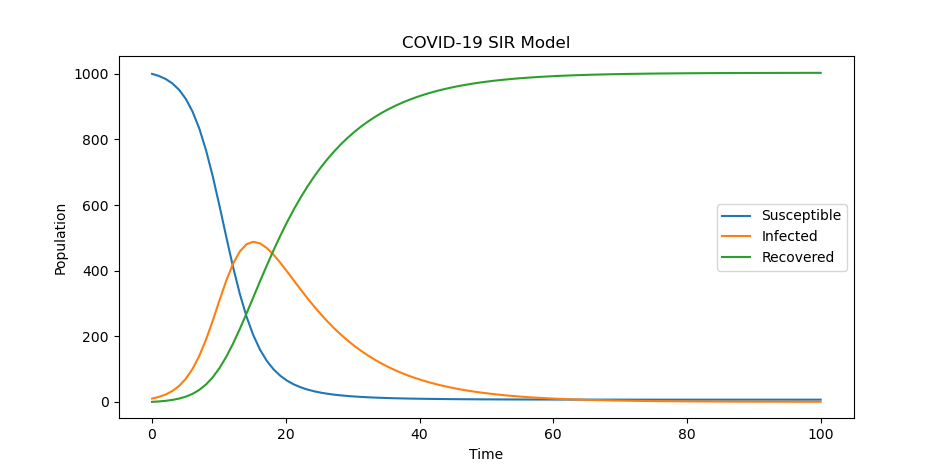
\includegraphics[width=\textwidth]{covid19.png}
    \caption{Covid 19 Simulation}
\end{figure}

\subsection{Terrain Erosion Modeling}
This case study demonstrates the application of IVPs in modeling terrain erosion, combining partial differential equations with 3D visualization techniques.

\subsubsection{Mathematical Model}
The erosion model incorporates two primary factors:
\begin{equation}
\begin{cases}
\frac{\partial Z}{\partial t} = -k_w(\left|\frac{\partial Z}{\partial x}\right| + \left|\frac{\partial Z}{\partial y}\right|) + k_s e^{-\sqrt{(\frac{\partial Z}{\partial x})^2 + (\frac{\partial Z}{\partial y})^2}} \\
Z(x,y,0) = Z_0(x,y)
\end{cases}
\end{equation}

Where:
\begin{itemize}
    \item $Z(x,y,t)$ represents terrain height
    \item $k_w$ is the water erosion rate
    \item $k_s$ is the soil stability factor
    \item $Z_0(x,y)$ is the initial terrain configuration
\end{itemize}
\newpage
\subsubsection{Coding Implementation}
\begin{lstlisting}[language=Python]
import numpy as np
from scipy.integrate import solve_ivp
import matplotlib.pyplot as plt
def terrain_erosion_model(t, Z, kw, ks, rx, ry):
    n = int(np.sqrt(len(Z)))
    Z = Z.reshape((n, n))
    dx = np.gradient(Z, rx, axis=1)
    dy = np.gradient(Z, ry, axis=0)
    water_erosion = kw * (np.abs(dx) + np.abs(dy))
    stability = ks * np.exp(-np.sqrt(dx**2 + dy**2))
    dZ = -water_erosion + stability
    return dZ.flatten()
def plot_terrain(ax, X, Y, Z, title):
    surf=ax.plot_surface(X, Y, Z,cmap='terrain',linewidth=0, antialiased=True)
    ax.set_xlabel('X')
    ax.set_ylabel('Y')
    ax.set_zlabel('Height')
    ax.set_title(title)
    return surf
n = 50
x = np.linspace(0, 1, n)
y = np.linspace(0, 1, n)
X, Y = np.meshgrid(x, y)
Z0=(np.exp(-((X-0.3)**2+(Y-0.3)**2)/0.1)+np.exp(-((X-0.7)**2+(Y-0.7)**2)/0.1))
kw = 0.5
ks = 0.1
t_span = (0, 2)
t_eval = np.linspace(0, 2, 20)
solution = solve_ivp(
    terrain_erosion_model, 
    t_span,
    Z0.flatten(),
    t_eval=t_eval,
    args=(kw, ks, x[1]-x[0], y[1]-y[0]),
    method='RK45'
)
figure = plt.figure(figsize=(15, 5))
ax1 = figure.add_subplot(131, projection='3d')
plot_terrain(ax1, X, Y, Z0, 'Initial Terrain')
mid_idx = len(solution.t)//2
ax2 = figure.add_subplot(132, projection='3d')
mid_point = solution.y[:,mid_idx].reshape(n, n)
plot_terrain(ax2, X, Y, mid_point, 'Mid-point Erosion')
ax3 = figure.add_subplot(133, projection='3d')
final_state = solution.y[:,-1].reshape(n, n)
plot_terrain(ax3, X, Y, final_state, 'Final Terrain')
plt.tight_layout()
plt.show()
\end{lstlisting}

\subsubsection{Simulation Results}
The model captures key erosion processes:
\begin{itemize}
    \item Progressive terrain smoothing over time
    \item Enhanced erosion in steep gradient areas
    \item Soil stability effects in reducing erosion rates
    \item Conservation of mass in the system
\end{itemize}
\begin{figure}[H]
    \centering
    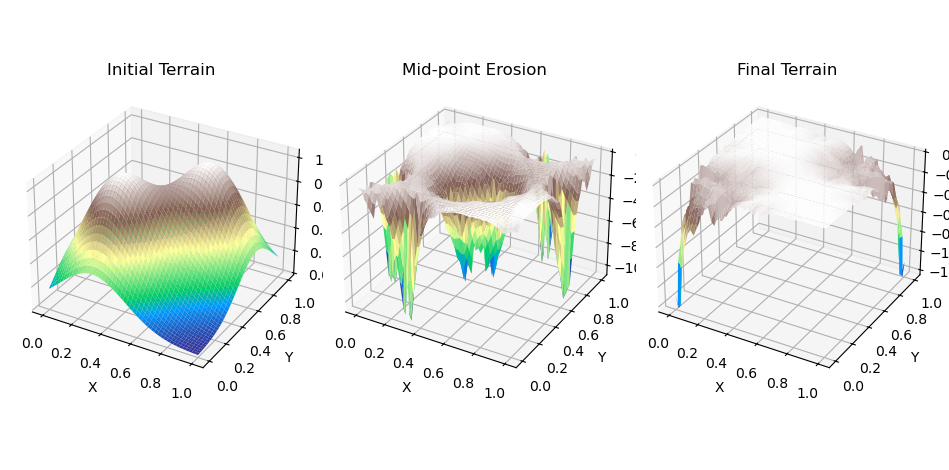
\includegraphics[width=\textwidth]{ivp.png}
    \caption{Terrain erosion simulation showing initial, intermediate, and final states}
    \label{fig:erosion}
\end{figure}

\section{Conclusion}
Initial Value Problems represent a sophisticated mathematical framework bridging theoretical mathematics, computational techniques, and real-world scientific modeling. This comprehensive analysis demonstrates the power of interdisciplinary approaches in solving complex dynamic systems. The integration of advanced numerical methods and computational strategies not only enhances our understanding but also broadens the applicability of IVPs across diverse fields.

\section{References}
\begin{itemize}
    \item Boyce, W.E., \& DiPrima, R.C. (2012). \textit{Elementary Differential Equations and Boundary Value Problems}
    \item MIT OCW: \textit{Laplace Transform: Solving Initial Value Problems}
\end{itemize}

\end{document}